%%%%%%%%%%%%%%%%%%%%%%%%%%%%%%%%%%%%%%%%
% Compact Laboratory Book
% LaTeX Template
% Version 1.0 (4/6/12)
%
% This template has been downloaded from:
% http://www.LaTeXTemplates.com
%
% Original author:
% Joan Queralt Gil (http://phobos.xtec.cat/jqueralt) using the labbook class by
% Frank Kuster (http://www.ctan.org/tex-archive/macros/latex/contrib/labbook/)
%
% License:
% CC BY-NC-SA 3.0 (http://creativecommons.org/licenses/by-nc-sa/3.0/)
%
% Important note:
% This template requires the labbook.cls file to be in the same directory as the
% .tex file. The labbook.cls file provides the necessary structure to create the
% lab book.
%
% The \lipsum[#] commands throughout this template generate dummy text
% to fill the template out. These commands should all be removed when 
% writing lab book content.
%
% HOW TO USE THIS TEMPLATE 
% Each day in the lab consists of three main things:
%
% 1. LABDAY: The first thing to put is the \labday{} command with a date in 
% curly brackets, this will make a new section showing that you are working
% on a new day.
%
% 2. EXPERIMENT/SUBEXPERIMENT: Next you need to specify what 
% experiment(s) and subexperiment(s) you are working on with a 
% \experiment{} and \subexperiment{} commands with the experiment 
% shorthand in the curly brackets. The experiment shorthand is defined in the 
% 'DEFINITION OF EXPERIMENTS' section below, this means you can 
% say \experiment{pcr} and the actual text written to the PDF will be what 
% you set the 'pcr' experiment to be. If the experiment is a one off, you can 
% just write it in the bracket without creating a shorthand. Note: if you don't 
% want to have an experiment, just leave this out and it won't be printed.
%
% 3. CONTENT: Following the experiment is the content, i.e. what progress 
% you made on the experiment that day.
%
%%%%%%%%%%%%%%%%%%%%%%%%%%%%%%%%%%%%%%%%%

%----------------------------------------------------------------------------------------
%	PACKAGES AND OTHER DOCUMENT CONFIGURATIONS
%----------------------------------------------------------------------------------------                               

% \UseRawInputEncoding

\documentclass[fontsize=11pt, % Document font size
                             paper=letter, % Document paper type
                             %twoside, % Shifts odd pages to the left for easier reading when printed, can be changed to oneside
                             openany, % chapters can start on any page
                             captions=tableheading,
                             index=totoc,
                             hyperref]{labbook}

%\documentclass[idxtotoc,hyperref,openany]{labbook} % 'openany' here removes the
  
\usepackage[bottom=10em]{geometry} % Reduces the whitespace at the bottom of the page so more text can fit

\usepackage[english]{babel} % English language
\usepackage{lipsum} % Used for inserting dummy 'Lorem ipsum' text into the template

\usepackage[utf8]{inputenc} % Uses the utf8 input encoding
\usepackage[T1]{fontenc} % Use 8-bit encoding that has 256 glyphs

\usepackage[osf]{mathpazo} % Palatino as the main font
\linespread{1.05}\selectfont % Palatino needs some extra spacing, here 5% extra
\usepackage[scaled=.88]{beramono} % Bera-Monospace
\usepackage[scaled=.86]{berasans} % Bera Sans-Serif

\usepackage{booktabs,array} % Packages for tables

\usepackage{amsmath} % For typesetting math
\usepackage{graphicx} % Required for including images
\usepackage{etoolbox}
\usepackage[norule]{footmisc} % Removes the horizontal rule from footnotes
\usepackage{lastpage} % Counts the number of pages of the document
\usepackage{float}
\usepackage{fancyvrb}



\usepackage[dvipsnames]{xcolor}  % Allows the definition of hex colors
\usepackage{epstopdf}
\epstopdfsetup{suffix={}}
\definecolor{titleblue}{rgb}{0.16,0.24,0.64} % Custom color for the title on the title page
\definecolor{linkcolor}{rgb}{0,0,0.42} % Custom color for links - dark blue at the moment

\addtokomafont{title}{\Huge\color{titleblue}} % Titles in custom blue color
\addtokomafont{chapter}{\color{OliveGreen}} % Lab dates in olive green
\addtokomafont{section}{\color{Sepia}} % Sections in sepia
\addtokomafont{pagehead}{\normalfont\sffamily\color{gray}} % Header text in gray and sans serif
\addtokomafont{caption}{\footnotesize\itshape} % Small italic font size for captions
\addtokomafont{captionlabel}{\upshape\bfseries} % Bold for caption labels
\addtokomafont{descriptionlabel}{\rmfamily}
\setcapwidth[c]{10cm} % Center align caption text
\setkomafont{footnote}{\sffamily} % Footnotes in sans serif

\deffootnote[4cm]{4cm}{1em}{\textsuperscript{\thefootnotemark}} % Indent footnotes to line up with text

\DeclareFixedFont{\textcap}{T1}{phv}{bx}{n}{1.5cm} % Font for main title: Helvetica 1.5 cm
\DeclareFixedFont{\textaut}{T1}{phv}{bx}{n}{0.8cm} % Font for author name: Helvetica 0.8 cm

\usepackage[nouppercase,headsepline]{scrpage2} % Provides headers and footers configuration
\pagestyle{scrheadings} % Print the headers and footers on all pages
\clearscrheadfoot % Clean old definitions if they exist

\automark[chapter]{chapter}
\ohead{\headmark} % Prints outer header

\setlength{\headheight}{25pt} % Makes the header take up a bit of extra space for aesthetics
\setheadsepline{.4pt} % Creates a thin rule under the header
\addtokomafont{headsepline}{\color{lightgray}} % Colors the rule under the header light gray

\ofoot[\normalfont\normalcolor{\thepage\ |\  \pageref{LastPage}}]{\normalfont\normalcolor{\thepage\ |\  \pageref{LastPage}}} % Creates an outer footer of: "current page | total pages"

% These lines make it so each new lab day directly follows the previous one i.e. does not start on a new page - comment them out to separate lab days on new pages
\makeatletter
\patchcmd{\addchap}{\if@openright\cleardoublepage\else\clearpage\fi}{\par}{}{}
\makeatother
\renewcommand*{\chapterpagestyle}{scrheadings}

% These lines make it so every figure and equation in the document is numbered consecutively rather than restarting at 1 for each lab day - comment them out to remove this behavior
\usepackage{chngcntr}
\counterwithout{figure}{labday}
\counterwithout{equation}{labday}

% Hyperlink configuration
\usepackage[
    pdfauthor={Brian Lauer and Elliot Watkins}, % Your name for the author field in the PDF
    pdftitle={Laboratory Journal}, % PDF title
    pdfsubject={labNotebookSeniorProject1}, % PDF subject
    bookmarksopen=true,
    linktocpage=true,
    urlcolor=linkcolor, % Color of URLs
    citecolor=linkcolor, % Color of citations
    linkcolor=linkcolor, % Color of links to other pages/figures
    backref=page,
    pdfpagelabels=true,
    plainpages=false,
    colorlinks=true, % Turn off all coloring by changing this to false
    bookmarks=true,
    pdfview=FitB]{hyperref}

\usepackage[stretch=10]{microtype} % Slightly tweak font spacing for aesthetics

\usepackage[framed,numbered,autolinebreaks,useliterate]{mcode}
\usepackage{todonotes}

%\setlength\parindent{0pt} % Uncomment to remove all indentation from paragraphs

%----------------------------------------------------------------------------------------
%	DEFINITION OF EXPERIMENTS
%----------------------------------------------------------------------------------------

% Template: \newexperiment{<abbrev>}[<short form>]{<long form>}
% <abbrev> is the reference to use later in the .tex file in \experiment{}, the <short form> is only used in the table of contents and running title - it is optional, <long form> is what is printed in the lab book itself

\newexperiment{example}[Example experiment]{This is an example experiment}
\newexperiment{example2}[Example experiment 2]{This is another example experiment}
\newexperiment{example3}[Example experiment 3]{This is yet another example experiment}

\newsubexperiment{subexp_example}[Example sub-experiment]{This is an example sub-experiment}
\newsubexperiment{subexp_example2}[Example sub-experiment 2]{This is another example sub-experiment}
\newsubexperiment{subexp_example3}[Example sub-experiment 3]{This is yet another example sub-experiment}

%----------------------------------------------------------------------------------------
\newcommand{\HRule}{\rule{\linewidth}{0.5mm}} % Command to make the lines in the title page

\setlength\parindent{0pt} % Removes all indentation from paragraphs

\begin{document}

%----------------------------------------------------------------------------------------
%	TITLE PAGE
%----------------------------------------------------------------------------------------
%\frontmatter % Use Roman numerals for page numbers

%\begin{center}

%

\title{
\begin{center}
\href{http://www.bradley.edu}{
\includegraphics[height=0.5in]{figs/logoBU1-Print}}
\vskip10pt
\HRule \\[0.4cm]
{\Huge \bfseries Laboratory Notebook \\[0.5cm] \Large Development of an Intelligent Building Energy Management System}\\[0.4cm] % Degree
\HRule \\[1.5cm]
\end{center}
}
\author{\Huge Brian Lauer and \Huge Elliot Watkins \\ \\\Large blauer@mail.bradley.edu, ejwatkins@mail.bradley.edu} % Your name and email address
\date{Beginning September 14, 2020} % Beginning date
\maketitle

%\maketitle % Title page

\printindex
\tableofcontents % Table of contents
\newpage % Start lab look on a new page

\begin{addmargin}[0cm]{0cm} % Makes the text width much shorter for a compact look

\pagestyle{scrheadings} % Begin using headers

%----------------------------------------------------------------------------------------
%	LAB BOOK CONTENTS
%----------------------------------------------------------------------------------------
r. 
\labday{Monday, September 14, 2020}

\experiment{Meeting Minutes}
BL \\
Today, in the meeting with Dr. Miah, we kicked off the project involving development of a building enery management platform. A Github repository was created for the project which will also be paired with a corresponding Google Drive titled "seniorProject1-2020-21". On Tuesdays and Thursdays, we will have lab time from 8am to 11am and weekly meetings with the advisor from 4pm to 5pm on Mondays this semester. The lab times are devoted specifically for work rather than research or documentation. Before coming to lab, work must be cut out for both of us.

\experiment{Homework}
BL\\
This document was created and pushed to the Github repository for both of us to use. For better portability, one of the laptops previously used for research on this project was wiped clean and LUbuntu was installed. As of now, most of the code developed for the platform was done on a desktop PC dual-booted with Ubuntu Linux and Windows 10. To be able to move between lab and home easily, a more ideal situation is to use a dedicated laptop with Linux installed. Because the USB drive used to install Linux was previously formatted with Ubuntu 18.04, the diskpart utility was used with the following commands:
\begin{Verbatim}
select disk 1
clean 
create partition primary
format quick
\end{Verbatim}
The Startup Disk Creator GUI program on Linux was utilized to flash the LUbuntu 64-bit desktop iso file on to the USB-thumb drive. The commands \texttt{sudo apt-get update} and \texttt{sudo apt-get upgrade} were run on the laptop to perform necessary upgrades and updates. Lastly, \texttt{sudo apt-get install git} was used to install git. Another package installed was \texttt{textlive-full} to compile latex with all the necessary packages.
%-------------------------------------------

\labday{Monday, September 21, 2020}

\experiment{Meeting Minutes}
BL\\
In the meeting with Dr. Miah, Dr. Miah pointed out that templates are available in the Google Drive for the lab notebook and other deliverables which we did not realize. In the System Level Requirements document (the first deliverable) we must replace the current block diagram with the drawing of the house connected to a microgrid. Inside, the home will be a block of the BEMS core which will connect to various IoT devices in the building. The controllable loads in the building including devices like lights, appliances (including dishwashers, washing machines), and smart plugs. Examples of uncontrollable loads include desktop PCs, laptops, thermistors, and microwaves. In a potential future research project, connectivity with a microgrid may be possible, so powerlines representing the main grid will be connecting the house to a microgrid through a PCC (Point of Common Coupling). In the current version of the diagram, the file is simply too large as it contains many images from the Internet. This will be redrawn in inkscape with custom figures to reduce the file size.
\smallbreak\noindent
The final outcome of the project will be
\begin{itemize}
\item Laptop running in the IoT lab or office
\item 2-3 devices in office/lab can be controlled succesfully
\item System should recognize the devices immediately upon connection to the network
\item Algorithm implemented to help improve energy efficiency
\end{itemize}
As a part of the first deliverable, three modes of operation will be declared including
\begin{itemize}
\item Device search mode
\item Device operation mode
\item Third mode to be determined
\end{itemize}
The sections of the deliverable will be
\begin{itemize}
\item Problem Statement
\item System Architecture
\item Block Diagram
\item Modes of Operation
\end{itemize}
Another point brought up is whether an energy efficient algorithm should be included in the software. Dr. Miah said yes. This will possibly help to boost the complexity of the project and improve the usefuleness of the platform. This algorithm will have to be determined.
\smallbreak\noindent
As of today, we should both be writing code on Tuesdays and Thursdays or possibly on our own, and we can both use code written for the research project. The split should be 50/50 so a Gantt chart will need to be made. 
%--------------------------------------------------------------------c--------------------

\labday{Tuesday, September 22, 2020}

\experiment{Lab work}

BL\\
Elliot and I met over Zoom to work on getting a new Github repo setup for the senior project code specifically. Although Dr. Miah mentioned in the meeting that the code should be on Github, we simply will periodically upload the zipped Github project to the Drive to the implementation/ folder. I copied over the files from the research to the new Github repo cloned locally on my Linux laptop. After running the \texttt{install.sh} script, the installation failed as the Linux laptop I am using is running Python3.5 rather than Python3.6 which is required for f-string support. An example of a line that failed is shown in the figure below:
\begin{figure}[H]
\centering
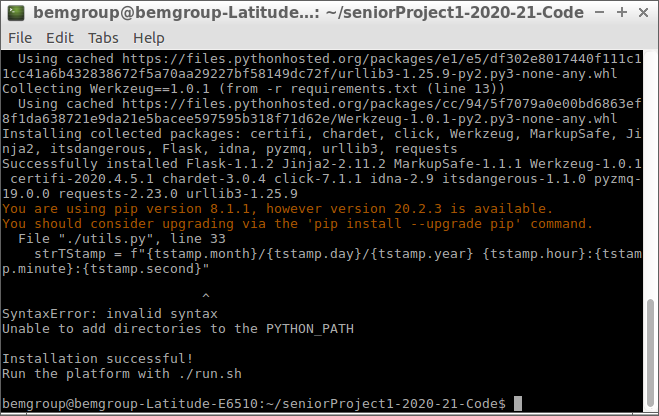
\includegraphics[scale=0.6]{figs/img/installSyntaxError}
\caption{f string error in \texttt{utils.py}}
\end{figure}
A simple solution to this problem was simply using string concatenation:
\begin{Verbatim}
strTStamp = str(tstamp.month) + "/" + str(tstamp.day) + "/" + str(tstamp.year) + " "
strTStamp += str(tstamp.hour) + ":" + str(tstamp.minute) + ":" + str(tstamp.second)
\end{Verbatim}
Further changes were made in the \texttt{ControlAgent.py} and \texttt{DiscoveryAgent.py} files. In particular, the line in \texttt{subscribe} to connect to the server acting as the central exchange to process publish/subscribe messages between the web server backend and agents listening for subscriptions was altered to support string concatenation. After these alterations to the source code were made, the platform was succesfully started. However, it is clear that no messages published to the server were received by both either the \texttt{ControlAgent} or \texttt{DiscoveryAgent} which will need to be debugged in the next lab or possilby before. This is evident as the terminals showing the debug output of each agent not indicating any messages received. Messages should be published via the publish function in the file \texttt{PROJECT\_DIR/WebServer/pubsub.py}. All these problems must be fixed to allow the ActiveDevices page to discover and connect to devices.
\end{addmargin}
%--------------------------------------------------------------------c--------------------

\labday{Monday, September 28, 2020}

\experiment{Meeting Minutes}
EW\\
{\bf Agenda:}
How to auto-detect devices on the network (interrupt or polling)? We were thinking of constantly pinging the network for supported devices in an infinite loop. Is there a way for a device to send a request to the server once it has joined the network?

We would like to add support for a smart power meter that can connect to WiFi, so power data for the entire building/house can be shown in the UI. What would you recommend in terms of a cost-effective solution? I found a device called the Sense Energy Monitor that can send data over wifi to an mobile or web app that comes with the device. The device itself connects to the electrical panel of a house. However, it is quite expensive at a price of 299 dollars.

Does the platform still need to be agent-based like BEMOSS? 

{\bf Discussion:}
For auto-detecting, we need to research how to create an interrupt. IF that turns out to be impossible, we will try to replicate Windows trying to find bluetooth devices. It will be a poling process that is explicitly demanded by the user.



\end{document}


%%% Local Variables:
%%% mode: latex
%%% TeX-master: t
%%% End:
